\begin{figure*}
\centering
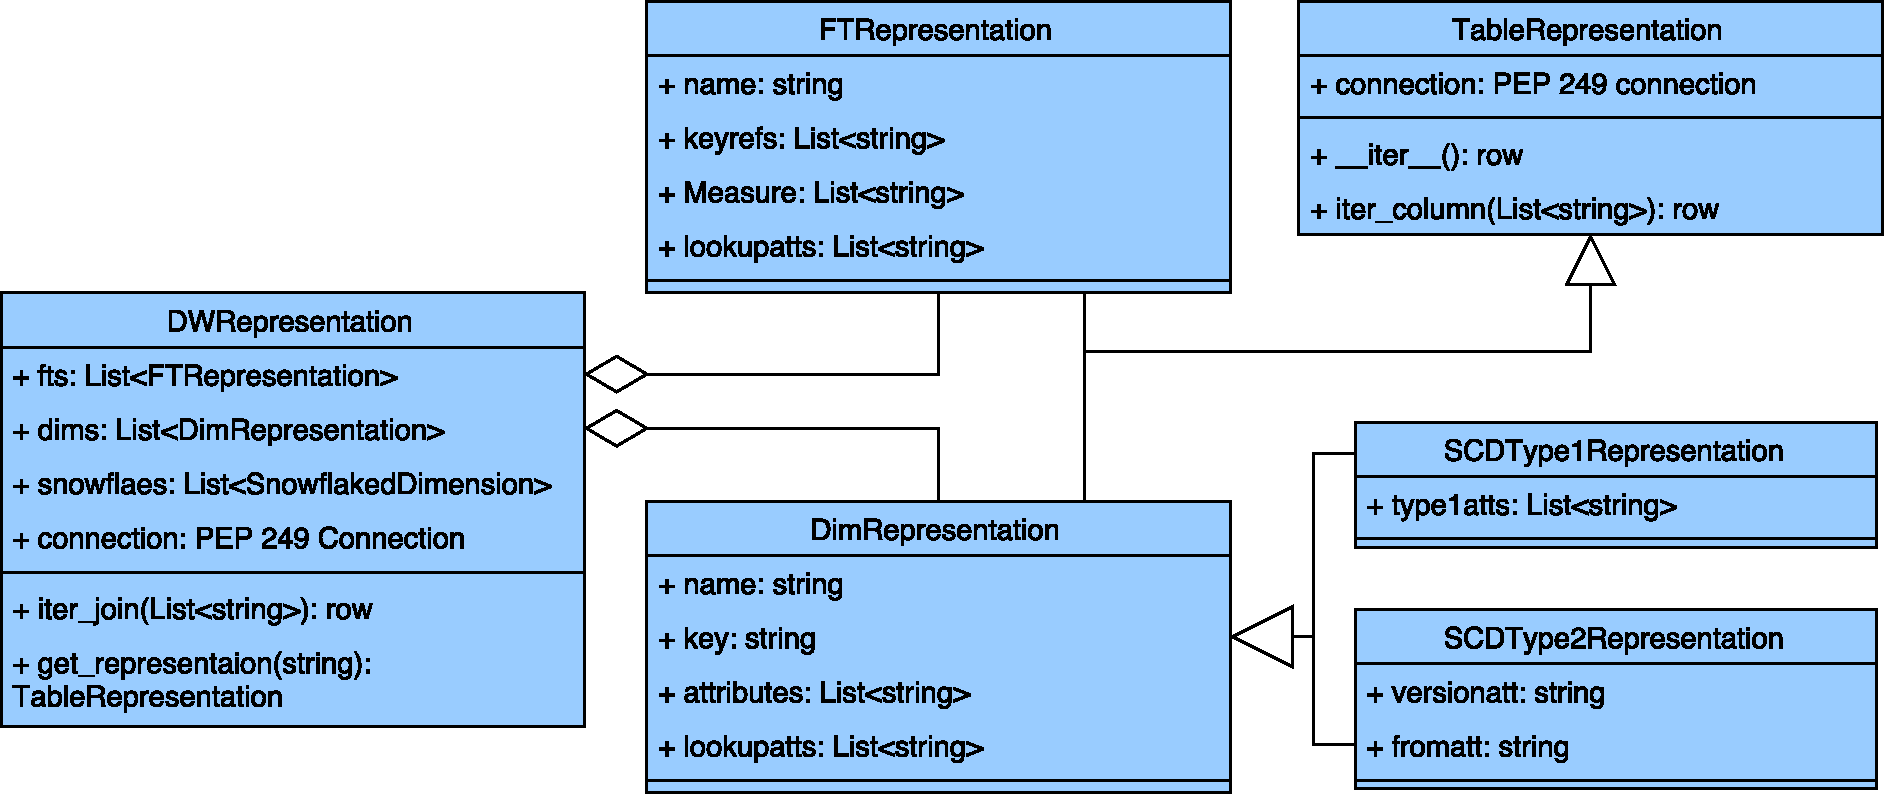
\includegraphics[width=0.9\textwidth]{figures/dwrep_uml.pdf}
\caption{UML diagram of the intermediate representations}
\label{fig:dwrep}
\end{figure*}

\section{Intermediate Data Representations}\label{sect:interdatarep}

This section will go into details about the different intermediate data representations used by the predicates. These representations are meant to standardize input to the predicates, so that the DW may be easily accessed. There are two main intermediate data representations \textit{DWRepresentation} and \textit{TableRepresentation}. DWRepresentation represents the DW as a whole, and the TableRepresentation and its subclasses represent the DWs tables. A UML diagram of the intermediate data representations can be seen in \Cref{fig:dwrep}. Both classes are involved in the execution of the DWPopulator class as described in \Cref{sec:dwpopulator}. The metadata stored in both classes is used when dynamically creating SQL queries in the predicates. However both also contain methods that assist in extracting data, so that it may be processed using python. 

\subsection{DWRepresentation}
The \textit{DWRepresentation} is a container object and includes information about the DW's schema and contents. A DWRepresentation object is created by the \textit{RepresentationMaker} by aggregating a number of \textit{TableRepresentations}.

The DWRepresentation has the following main attributes:

\begin{description}
\item[Dimensions] List of \textit{DimRepresentations} detailing each dimension in the DW along with their metadata.
\item[FactTables] List of fact tables in the DW along with metadata.
\item[Snowflakes] List of Snowflaked dimensions. This is used to construct the DW schema.
\item[Connection] A PEP 249 connection object for accessing the DW, so that we may query it for data later on.
\end{description}
The object also provides methods for connecting to and extracting data from the DW. Data can be extracted in one of two ways.

By supplying the name of a table to the get\_data\_representation method, it will return the corresponding TableRepresentation object. DWRepresentaion also supplies the iter\_join method. Giving this method a number of table names as input, it will return an iterable. This way we can extract and  iterate over the natural join of the given tables as a list of dictionaries within python. 

During instantiation, the DWRepresentation also find the DW’s schema . This is done using the \_find\_structure method. For each fact table, we register all dimensions, which it may be naturally joined with. That is, an attribute in the fact table’s keyrefs set is the same as the primary key of a dimension. In the case of our snowflaked dimensions, a fact table may only have a foreign key to the snowflake root. Dimensions within snowflakes are the only ones allowed to have a foreign key to other dimensions. Doing this lookup for each fact table, we end up with a dictionary, where the keys are fact table names pointing to sets of dimensions. An example would be \{ft:(A,B)\}, which states that the fact table ft has foreign keys to the dimensions A and B. To this dictionary we add the internal reference information of each snowflaked dimension. Thus it also contains keys for dimensions with foreign keys to other dimensions within snowflakes. Because how we find the structure, pairs of referring and referred tables need to be joinable through a natural join. 

\subsection{TableRepresentation}
\textit{TableRepresentation} is a superclass used for representing data from specific tables. The subclasses contains metadata regarding the tables themselves, such as the table name, attributes etc. A subclass is instantiated by taking an instance of its corresponding pygrametl table as input. It then copies the relevant metadata and PEP 249 connection object into itself.

The currently supported table types are:

\begin{itemize}
\item Dimension
\item Type 1 Slowly Changing Dimensions
\item Type 2 Slowly Changing Dimensions
\item FactTable
\end{itemize}

Any dimension or fact table found in a pygrametl program is simply represented in a DimensionRepresentation or FactTableRepresentation respectively. Special subclasses are made for the slowly changing dimensions, as they contain unique information important during the execution of certain predicates.

When working with DW data in python, rather than SQL, the data within a specific table can be extracted  by iterating over the TableRepresentation as a list of dictionaries. This queries the DW and yields a single row at a time. It also has the itercolumns method, which allows for only a specified subset of table columns to be iterated in the same manner.

